\documentclass[12pt,twoside,notitlepage]{report}
\usepackage{a4wide}
\usepackage{graphicx}


\raggedbottom                           % try to avoid widows and orphans
\sloppy
\clubpenalty1000%
\widowpenalty1000%

\addtolength{\oddsidemargin}{6mm}       % adjust margins
\addtolength{\evensidemargin}{-8mm}

\renewcommand{\baselinestretch}{1.1}    % adjust line spacing to make
                                        % more readable

\parindent 0pt
\parskip 6pt

\begin{document}

\pagestyle{empty}

\vspace*{60mm}
\begin{center}
\Huge
{\bf Project Proposal}
\end{center}

\cleardoublepage

\section*{Introduction and Description of the Work}

As computer graphics technology has advanced over the years, original artistic styles have evolved with it.

Early technology was scanline-based, capable of drawing simple blocks of colour. As the fidelity demanded of graphics increased, specialised hardware that could deal with complex two-dimensional scenes was developed; however, it was still limited in many ways. Two widespread limitations were that higher-speed graphics modes restricted the palette of colours that could be displayed per 2D object (`sprite'), and the output resolution of the hardware was relatively tiny compared to today's technology (for example, $320\times240$ pixels was commonly used).

\begin{figure}[h!]
\centering
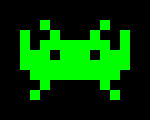
\includegraphics{spaceinvadersprite}
\caption{An early example of pixel art, from Space Invaders (Taito, 1978)}
\end{figure}

The combination of these restrictions led to the rise of an art style now known as `pixel art'. This was characterised by bright colours with distinct levels of shading, dark single-pixel outlines that contrasted against often busy backgrounds, and thanks to the low resolution, the use of single pixel positioning to show small details. As the style evolved, further techniques were invented, such as the use of several shades of the same outline colour to make edges appear smooth, and `dithering', a pixel-grid checkerboard pattern between two shades of a colour to give the illusion of a third intermediate shade.

\begin{figure}[h!]
\centering
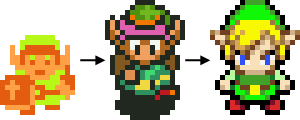
\includegraphics{linksprite}
\caption{The evolution of pixel art, from The Legend of Zelda series (Nintendo, 1986-2005)}
\end{figure}

Eventually, 2D graphics hardware was replaced by 3D hardware, and pixel art fell out of general use due to the requirement to painstakingly hand-draw pixel by pixel, for each of dozens or even hundreds of frames of animation. In terms of artistic effort required, 3D is much easier to work with for complicated scenes and characters. However, with the rise of mobile devices with limited graphics hardware and users looking fondly back at the computer games of their past, pixel art remains a popular art style.

The project intends to combine the ease of 3D animation with the aesthetics of pixel art, by using modern graphics technology to render 3D models in the style of pixel art. As the style is mainly used in computer games, the code will perform this in real time, allowing developers to use the pixel art style dynamically in a way that is impossible with hand-drawn art.

\section*{Starting Point}

I worked with GLSL, specifically fragment shaders, on a project at the University Computer Lab in Summer 2013, and also have some experience writing OpenGL code. I have drawn pixel art graphics in the past and consider myself to be experienced with the art style.

\begin{figure}[h!]
\centering
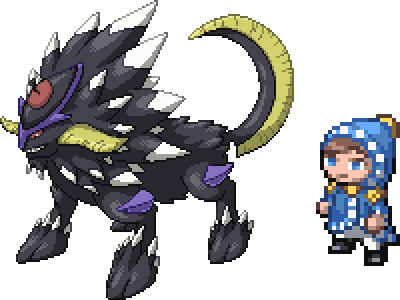
\includegraphics{examplesprite}
\caption{Examples of pixel art graphics I have drawn}
\end{figure}

\section*{Substance and Structure of the Project}

The main aim of the project is to implement OpenGL and GLSL code to render 3D models in a 2D pixel art-like style. The project will allow a 3D scene and corresponding animations to be loaded from a file, then render it to the screen at a smooth framerate. At the beginning of the project, I will choose a programming language and a corresponding OpenGL binding to use. I am considering C++, Java, and WebGL.

I will decide on a file type to use for loading 3D models. There are many file types designed for this purpose; the chosen type must support texturing, different materials, and animation. Ideally, it will be simple to parse so I can implement the parser quickly.

Next, I will need to write a skeleton renderer. At the beginning of the project, this will render the model using the standard Phong shading algorithm. As the project progresses, I will gradually implement custom rendering code instead; this approach will allow me to see the output of my code as I implement it. This means I can spot any bugs I insert quickly, and fix them.

As pixel art uses a limited colour palette, I will need to implement an algorithm to select a palette from the input model and texture data. This will need to generate new colours for areas of the model in shade and directly in the light. As stated above, I will also include the option to specify a palette for the model manually; this will be added first, allowing me to focus on the rendering code. I will return to the problem of selecting a palette later in the project, using the median cut algorithm as a starting point.

The part of the project that applies block shading will be relatively quick to write, as it is similar to the existing `cel shading' algorithm; it differs mainly in that it needs to select colours from a predefined palette instead of performing a 1D texture lookup. It will need to support ordinary 2D texture mapping. I will also implement dithering in this step, looking at the material properties and surface normals of the model to choose areas where the effect should be used. All of this will be implemented solely using fragment shaders.

\begin{figure}[h!]
\centering
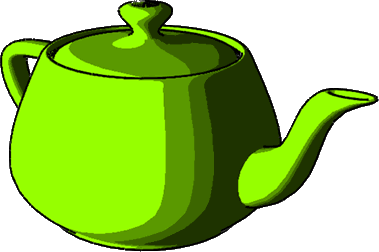
\includegraphics{celshading}
\caption{An example of cel shading (from Wikimedia Commons)}
\end{figure}

\begin{figure}[h!]
\centering
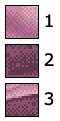
\includegraphics{dithering}
\caption{Examples of types of dithering (from Wikimedia Commons)}
\end{figure}

Single pixel outlines can also be implemented using a fragment shader; note that outlines occur when a front-facing polygon meets a back-facing polygon, so an outline can be drawn by rendering front-facing polygons as usual, then setting the depth test to allow fragments with an equal depth and rendering back-facing polygons. The front-facing polygon depth data still exists, so only pixels along edges will pass the depth test and be rendered.

Line smoothing will be implemented by extending the above with a vertex shader passing data to a geometry shader. The edges to be outlined must be identified on a separate pass before the model is shaded; then, the geometry shader can subdivide polygons along the edge to ensure the pixels along the edge appear smooth. Another fragment shader will be used to add further shading to the outline.

\begin{figure}[h!]
\centering

\includegraphics{linesmoothing}
\caption{An example of pixel art line smoothing. A curve rendered by a painting application is on the left, while a smoothed version is on the right.}
\label{fig:linesmoothing}
\end{figure}

The most difficult part will be to implement preservation of detail at small sizes and across frames; for example, if a detail ends up being smaller that a single pixel, it may not be rendered normally. This will be done by identifying details smaller than a threshold size (possibly depending on the type of detail; for example, one-pixel outlining means geometry details will need to be at least three pixels wide in order for the actual material colour to be visible), and using a geometry shader to expand them. Attention will need to be given to how it affects the surrounding area. At first, I will only consider geometry when looking for details; as an extension, I will try to take texture data into consideration too.

To evaluate the project, I will use two methods. Firstly, I will use an objective method to measure the real-time aspect. I will run the renderer on a number of devices with modern graphics hardware, and collect data on frame render time for scenes of varying complexity, both using standard Phong shading and my pixel art shader.

As the majority of the project concerns aesthetics, I will also use human experiments. I will ask subjects to compare images rendered with the project with images rendered in other ways. Some methods of evaluation I could use are:

\begin{itemize}

\item In order to test the visual appearance of my line smoothing algorithm, I will render the same model with and without line smoothing turned on. I will then ask test subjects to say which they prefer. I will make sure the images are shown in a random order.

\item Similarly, to test the appearance of dithering, I will render the same model with and without dithering enabled and ask test subjects to say which they prefer. Again, I will show the images in a random order.

\item To test detail preservation, I will create several models with easily recognisable detail, such as a texture that has text on it. Then, for each subject, I will render each model once at one of a number of different sizes and with detail preservation enabled or disabled; the number of models used must be small enough such that across all test subjects, each model is represented several times at each size and with detail preservation both enabled and disabled. I will ask the test subjects to identify (e.g. read) the details if possible. Collecting the results, I can measure how effective the algorithm is.

\item To test the overall capability of the project, I will display a character model rendered by my project next to pixel art of the same character hand-drawn by several different artists, and ask the test subjects to rank them in order of aesthetics.

\end{itemize}

\section*{Success Criterion}

The final deliverables of the project will be:

\begin{itemize}

\item A renderer application that allows the user to load a model file and change render settings

\item An algorithm that selects a colour palette of a given size to use based on the materials of a model

\item Highlights and shadowing in the pixel art style, including the use of dithering

\item Pseudo-antialiased and smoothed outlining, as demonstrated in figure~\ref{fig:linesmoothing}

\item Detail preservation when a model is rendered at small sizes

\end{itemize}

The criteria for the success of the project will be:

\begin{itemize}

\item The renderer must be able to render the Stanford dragon standard test model at a frame rate of at least 60 frames per second on both my desktop and laptop graphics processors (Nvidia GeForce GTX 560Ti and 765M respectively)

\begin{figure}[h!]
\centering
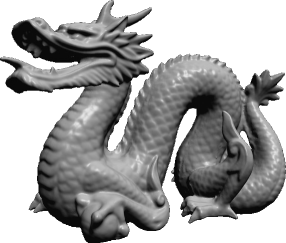
\includegraphics{stanforddragon}
\caption{A render of the Stanford dragon test model, consisting of several hundred thousand polygons.}
\end{figure}

\item The human experiment comparing rendered images with and without dithered shading should result in the dithered images being preferred in at least 70\% of the trials

\item The human experiment comparing rendered images with and without line smoothing should result in the line smoothed images being preferred in at least 70\% of the trials

\item The human experiment measuring the effectiveness of detail preservation should result in the detail preserved images being recognisable at smaller sizes than the non-detail preserved images in at least 70\% of the trials

\item The human experiment comparing my project's output with hand-drawn art should result in the rendered images being preferred over at least one hand-drawn image in at least 50\% of the trials

\end{itemize}

\section*{Timetable and Milestones}

\subsection*{Weeks 1 and 2 (26th October to 6th November)}

Refresh my knowledge of OpenGL and GLSL by skimming the OpenGL and GLSL reference manuals. Research similar shading algorithms such as cel shading. Decide on a language to use and a file type to load 3D models from.

\subsection*{Weeks 3 and 4 (7th November to 20th November)}

Plan and implement a simple renderer, using a Phong shader that will be replaced over the course of the project. Implement model loading.

\subsection*{Weeks 5 and 6 (21st November to 4th December)}

Implement loading of palettes from a text file. Add basic palette-limited shading, and start working on implementing dithering.

\subsection*{Weeks 7 and 8 (5th December to 18th December)}

Finish implementing dithering, and implement basic pixel outline rendering.

\subsection*{Weeks 9 and 10 (19th December to 1st January)}

Finish any unfinished sections from Michaelmas Term. Formally plan out human experiments, and find other pixel artists to make the hand-drawn art required for comparison.

Milestone: Basic pixel art rendering with dithering.

\subsection*{Weeks 11 and 12 (2nd January to 15th January)}

Start implementing outline smoothing geometry shader.

\subsection*{Weeks 13 and 14 (16th January to 29th January)}

Finish outline smoothing geometry shader, start implementing fragment shader.

\subsection*{Weeks 15 and 16 (30th January to 12th February)}

Finish outline smoothing fragment shader, implement automated palette selection.

Milestone: Pixel art rendering with smoothed outlines and automatically selected palettes.

\subsection*{Weeks 17 and 18 (13th February to 26th February)}

Start work on algorithm to preserve details across scaling and animation.

\subsection*{Weeks 19 and 20 (27th February to 12th March)}

Complete detail preservation algorithm. Find volunteers for human experiments.

\subsection*{Weeks 21 and 22 (13th March to 26th March)}

Finish any unfinished sections from Lent Term. Carry out human testing.

Milestone: Complete pixel art rendering and perform human testing.

\subsection*{Weeks 23 and 24 (27th March to 9th April)}

Plan out dissertation, start writing.

\subsection*{Weeks 25 and 26 (10th April to 23rd April)}

Continue writing dissertation, finish a first draft. Send draft to my supervisor for review and proofreading.

Milestone: First draft of dissertation sent to supervisor.

\subsection*{Weeks 27 and 28 (24th April to 7th May)}

Get feedback from supervisor by the middle of the fortnight, and incorporate any necessary changes. As the deadline is the 16th, there is over a week of leeway in case something goes wrong.

Milestone: Submit dissertation.

\section*{Resources Required}

The project will be implemented using the graphics library OpenGL and GLSL (the OpenGL Shading Language). As such, the project requires the availability of graphics hardware that supports these.

I am also intending to use my own laptop for the project (2.4GHz Core i7, GeForce GTX765M, 8GB RAM, 1TB solid state hybrid drive). As backup, I will use my desktop PC (3.4GHz Core i5, GeForce 560Ti, 8GB RAM, 1TB hard drive). Both computers have the graphics hardware required to implement the project.

As my main backup strategy, I will use the Git version control system, using the online service GitHub to store my files. In addition, I will back up any modified files daily on a USB drive and on my DropBox account.

\end{document}
